%%%%%%%%%%%%%%%%%%%%%%%%%%%%%%%%%%%%%%%%%%%%%%%%%%%%
% Document type, global settings, and packages
%%%%%%%%%%%%%%%%%%%%%%%%%%%%%%%%%%%%%%%%%%%%%%%%%%%%

\documentclass[12pt]{report}   %12 point font for Times New Roman
\usepackage[backend=bibtex, sorting=none, style=ieee]{biblatex}  %reference manager
\usepackage{microtype}
\usepackage{graphicx}  %for images and plots
\usepackage{listings}
\lstset{
  numbers=left, 
  firstnumber=1,
  numberfirstline=true
}
\usepackage[letterpaper, left=1.5in, right=1in, top=1in, bottom=1in]{geometry}
\usepackage{setspace}  %use this package to set linespacing as desired
\usepackage{times}  %set Times New Roman as the font
\usepackage[explicit]{titlesec}  %title control and formatting
\usepackage[titles]{tocloft}  %table of contents control and formatting
\usepackage{booktabs}
\usepackage[bookmarks=true, hidelinks]{hyperref}
\usepackage[page]{appendix}  %for appendices
\usepackage{rotating}  %for rotated, landscape images
\usepackage{ulem}  %for underlined section titles
% additional packages
\usepackage{blindtext}
\usepackage{mathtools}
\usepackage{algorithm,algpseudocode}
\usepackage[linguistics]{forest}
\usepackage[utf8]{inputenc}

%%%%%%%%%%%%%%%%%%%%%%%%%%%%%%%%%%%
% Bibliography
%%%%%%%%%%%%%%%%%%%%%%%%%%%%%%%%%%%

%Add your bibliography file here
\bibliography{references}

% prevent certain fields in references from printing in bibliography
\AtEveryBibitem{\clearfield{issn}}
\AtEveryBibitem{\clearlist{issn}}

\AtEveryBibitem{\clearfield{language}}
\AtEveryBibitem{\clearlist{language}}

\AtEveryBibitem{\clearfield{doi}}
\AtEveryBibitem{\clearlist{doi}}

\AtEveryBibitem{\clearfield{url}}
\AtEveryBibitem{\clearlist{url}}

\AtEveryBibitem{%
  \ifentrytype{online}
    {}
    {\clearfield{urlyear}\clearfield{urlmonth}\clearfield{urlday}}}

%%%%%%%%%%%%%%%%%%%%%%
% Start of Document
%%%%%%%%%%%%%%%%%%%%%%

\begin{document}
\doublespacing  %set line spacing

%%%%%%%%%%%%%%%%%%%%%%%%%%%%%%%%%%%%%
% Title Page
%%%%%%%%%%%%%%%%%%%%%%%%%%%%%%%%%%%%%

%% Define your thesis title, your name, your school, and your month and year of graduation here

\newcommand{\thesisTitle}{Automated Penetration Testing for PHP Web Applications}
\newcommand{\yourName}{Zixiang Zhu}
\newcommand{\yourSchool}{Georgia Institute of Technology}
\newcommand{\yourMonth}{November}
\newcommand{\yourYear}{2016}

%%%%%%%%%%%%%%%%%%%%%%%%%%%%%%%%%%%%%%%%%%%%%%%%%%%%%%%%%
% Do not edit these lines unless you wish to customize
% the template
%%%%%%%%%%%%%%%%%%%%%%%%%%%%%%%%%%%%%%%%%%%%%%%%%%%%%%%%%


\begin{titlepage}
\begin{center}

\begin{singlespacing}

\textbf{\MakeUppercase{\thesisTitle}}\\
\vspace{10\baselineskip}
A Dissertation\\
Presented to\\
The Academic Faculty\\
\vspace{3\baselineskip}
By\\
\vspace{3\baselineskip}
\yourName\\
% \vspace{3\baselineskip}
% In Partial Fulfillment\\
% of the Requirements for the Degree\\
% Doctor of Philosophy in the\\
% School of \yourSchool\\
\vspace{3\baselineskip}
Georgia Institute of Technology\\
\vspace{\baselineskip}
\yourMonth{} \yourYear{}
\vfill
Copyright \copyright{} \yourName{} \yourYear{}

\end{singlespacing}

\end{center}
\end{titlepage}



\currentpdfbookmark{Title Page}{titlePage}  %add PDF bookmark for this page

%%%%%%%%%%%%%%%%%%%%%%%%%%%%%%%%%%%%%
% Approval Page
%%%%%%%%%%%%%%%%%%%%%%%%%%%%%%%%%%%%%

% %% Define your committee members. If you have less than 6, simple delete/comment the unused lines

\newcommand{\committeeMemberOne}{Dr. Burdell, Advisor}
\newcommand{\committeeMemberOneDepartment}{School of Myths}
\newcommand{\committeeMemberOneAffiliation}{Georgia Institute of Technology}

\newcommand{\committeeMemberTwo}{Dr. Two}
\newcommand{\committeeMemberTwoDepartment}{School of Mechanical Engineering}
\newcommand{\committeeMemberTwoAffiliation}{Georgia Institute of Technology}

\newcommand{\committeeMemberThree}{Dr. Three}
\newcommand{\committeeMemberThreeDepartment}{School of Electrical Engineering}
\newcommand{\committeeMemberThreeAffiliation}{Georgia Institute of Technology}

\newcommand{\committeeMemberFour}{Dr. Four}
\newcommand{\committeeMemberFourDepartment}{School of Computer Science}
\newcommand{\committeeMemberFourAffiliation}{Georgia Institute of Technology}

\newcommand{\committeeMemberFive}{Dr. Five}
\newcommand{\committeeMemberFiveDepartment}{School of Public Policy}
\newcommand{\committeeMemberFiveAffiliation}{Georgia Institute of Technology}

\newcommand{\committeeMemberSix}{Dr. Six}
\newcommand{\committeeMemberSixDepartment}{School of Nuclear Engineering}
\newcommand{\committeeMemberSixAffiliation}{Georgia Institute of Technology}

\newcommand{\approvalDay}{11}
\newcommand{\approvalMonth}{January}
\newcommand{\approvalYear}{2000}

%%%%%%%%%%%%%%%%%%%%%%%%%%%%%%%%%%%%%%%%%%%%%%%%%%%%%%%%%
% Do not edit these lines unless you wish to customize
% the template
%%%%%%%%%%%%%%%%%%%%%%%%%%%%%%%%%%%%%%%%%%%%%%%%%%%%%%%%%


\begin{titlepage}
\begin{singlespacing}
\begin{center}

\textbf{\MakeUppercase{\thesisTitle}}\\
\vspace{10\baselineskip}

\end{center}
\vfill

%Define minipages, depending on how many authors there are
\ifdefined\committeeMemberFour

Approved by:
\vspace{2\baselineskip}		%adjust the number in front of "\baselineskip" for alignment

\begin{minipage}[b]{0.4\textwidth}
	
	\committeeMemberOne\\
	\committeeMemberOneDepartment\\
	\textit{\committeeMemberOneAffiliation}\\
	
	\committeeMemberTwo\\
	\committeeMemberTwoDepartment\\
	\textit{\committeeMemberTwoAffiliation}\\
	
	\committeeMemberThree\\
	\committeeMemberThreeDepartment\\
	\textit{\committeeMemberThreeAffiliation}\\
	
	\vspace{2\baselineskip}		%adjust the number in front of "\baselineskip" for alignment
	
\end{minipage}
\hspace{0.1\textwidth}
\begin{minipage}[b]{0.4\textwidth}
	
	\committeeMemberFour\\
	\committeeMemberFourDepartment\\
	\textit{\committeeMemberFourAffiliation}\\
	
	\ifdefined\committeeMemberSix
	\committeeMemberFive\\
	\committeeMemberFiveDepartment\\
	\textit{\committeeMemberFiveAffiliation}\\
	
	\committeeMemberSix\\
	\committeeMemberSixDepartment\\
	\textit{\committeeMemberSixAffiliation}\\
	
	Date Approved: \approvalMonth{} \approvalDay, \approvalYear
	\vspace{1\baselineskip}		%adjust the number in front of "\baselineskip" for alignment
	
	\else
	
	\committeeMemberFive\\
	\committeeMemberFiveDepartment\\
	\textit{\committeeMemberFiveAffiliation}\\
		
	Date Approved: \approvalMonth{} \approvalDay, \approvalYear
	\vspace{5\baselineskip}		%adjust the number in front of "\baselineskip" for alignment
	
	\fi
	
\end{minipage}

\else

\hspace{0.6\textwidth}
\begin{minipage}[b]{0.4\textwidth}
	
	Approved by:
	\vspace{2\baselineskip}		%adjust the number in front of "\baselineskip" for alignment
	
	\committeeMemberOne\\
	\committeeMemberOneDepartment\\
	\textit{\committeeMemberOneAffiliation}\\
	
	\committeeMemberTwo\\
	\committeeMemberTwoDepartment\\
	\textit{\committeeMemberTwoAffiliation}\\
	
	\committeeMemberThree\\
	\committeeMemberThreeDepartment\\
	\textit{\committeeMemberThreeAffiliation}\\
	
	\vspace{2\baselineskip}		%adjust the number in front of "\baselineskip" for alignment
	
	Date Approved: \approvalMonth{} \approvalDay, \approvalYear
	\vspace{\baselineskip}		%adjust the number in front of "\baselineskip" for alignment
	
\end{minipage}

\fi





\end{singlespacing}
\end{titlepage}


%%%%%%%%%%%%%%%%%%%%%%%%%%%%%%%%%%%%%
% Epigraph
%%%%%%%%%%%%%%%%%%%%%%%%%%%%%%%%%%%%%

% Define your quote and author for the epigraph here

\newcommand{\yourQuote}{Tests are stories we tell the next generation of programmers on a project.}
\newcommand{\yourAuthor}{Roy Osherove, The Art of Unit Testing: With Examples in .NET}

%%%%%%%%%%%%%%%%%%%%%%%%%%%%%%%%%%%%%%%%%%%%%%%%%%%%%%%%%
% Do not edit these lines unless you wish to customize
% the template
%%%%%%%%%%%%%%%%%%%%%%%%%%%%%%%%%%%%%%%%%%%%%%%%%%%%%%%%%

\begin{titlepage}
\begin{center}

\vspace*{\fill}
\yourQuote\\
\textit{\yourAuthor}
\vspace*{\fill}

\end{center}
\end{titlepage}



%%%%%%%%%%%%%%%%%%%%%%%%%%%%%%%%%%%%%
% Dedication
%%%%%%%%%%%%%%%%%%%%%%%%%%%%%%%%%%%%%

% % Define your dedication statement here

\newcommand{\yourDedication}{A great dedication goes here.}

%%%%%%%%%%%%%%%%%%%%%%%%%%%%%%%%%%%%%%%%%%%%%%%%%%%%%%%%%
% Do not edit these lines unless you wish to customize
% the template
%%%%%%%%%%%%%%%%%%%%%%%%%%%%%%%%%%%%%%%%%%%%%%%%%%%%%%%%%

\begin{titlepage}
\begin{center}

\vspace*{\fill}
\yourDedication\\
\vspace*{\fill}

\end{center}
\end{titlepage}


%%%%%%%%%%%%%%%%%%%%%%%%%%%%%%%%%%%%%
% Acknowledgments
%%%%%%%%%%%%%%%%%%%%%%%%%%%%%%%%%%%%%

% \pagenumbering{roman}
% \addcontentsline{toc}{chapter}{Acknowledgments}
% \setcounter{page}{5} % set the page number appropriately based on the number of intro pages
% \clearpage
\begin{centering}
\textbf{ACKNOWLEDGEMENTS}\\
\vspace{\baselineskip}
\end{centering}

%Insert your dedication text here
Lorem ipsum dolor sit amet, consectetur adipiscing elit, sed do eiusmod tempor incididunt ut labore et dolore magna aliqua. Ut enim ad minim veniam, quis nostrud exercitation ullamco laboris nisi ut aliquip ex ea commodo consequat. Duis aute irure dolor in reprehenderit in voluptate velit esse cillum dolore eu fugiat nulla pariatur. Excepteur sint occaecat cupidatat non proident, sunt in culpa qui officia deserunt mollit anim id est laborum.

\clearpage
%\pagenumbering{gobble}  %remove page number on summary page


%\addtocontents{toc}{\cftpagenumbersoff{chapter}} 

%\currentpdfbookmark{Acknowledgments}{acknowledgments}
%\addtocontents{toc}{\cftpagenumberson{chapter}} 

%%%%%%%%%%%%%%%%%%%%%%%%%%%%%%%%%%%%%
% Table of Contents
%%%%%%%%%%%%%%%%%%%%%%%%%%%%%%%%%%%%%

% Format for Table of Contents
\renewcommand{\cftchapdotsep}{\cftdotsep}  %add dot separators
\renewcommand{\cftchapfont}{\bfseries}  %set title font weight
\renewcommand{\cftchappagefont}{}  %set page number font weight
\renewcommand{\cftchappresnum}{Chapter }
\renewcommand{\cftchapaftersnum}{:}
\renewcommand{\cftchapnumwidth}{5em}
\renewcommand{\cftchapafterpnum}{\vskip\baselineskip} %set correct spacing for entries in single space environment
\renewcommand{\cftsecafterpnum}{\vskip\baselineskip}  %set correct spacing for entries in single space environment
\renewcommand{\cftsubsecafterpnum}{\vskip\baselineskip} %set correct spacing for entries in single space environment
\renewcommand{\cftsubsubsecafterpnum}{\vskip\baselineskip} %set correct spacing for entries in single space environment

%format title font size and position (this also applys to list of figures and list of tables)
\titleformat{\chapter}[display]
{\normalfont\bfseries\filcenter}{\chaptertitlename\ \thechapter}{0pt}{\MakeUppercase{#1}}

\renewcommand\contentsname{Table of Contents}

\begin{singlespace}
\tableofcontents
\end{singlespace}

\currentpdfbookmark{Table of Contents}{TOC}

\clearpage

%%%%%%%%%%%%%%%%%%%%%%%%%%%%%%%%%%%%%
% List of figures and tables
%%%%%%%%%%%%%%%%%%%%%%%%%%%%%%%%%%%%%

\addcontentsline{toc}{chapter}{List of Tables}
\begin{singlespace}
	\setlength\cftbeforetabskip{\baselineskip}  %manually set spacing between entries
	\listoftables
\end{singlespace}

\clearpage

\addcontentsline{toc}{chapter}{List of Figures}
\begin{singlespace}
\setlength\cftbeforefigskip{\baselineskip}  %manually set spacing between entries
\listoffigures
\end{singlespace}

\clearpage

%%%%%%%%%%%%%%%%%%%%%%%%%%%%%%%%%%%%%%%%%%%%%%%%%%%%%%%%%%%%%%%%%
% This is the Summary (abstract should be separate document)
%%%%%%%%%%%%%%%%%%%%%%%%%%%%%%%%%%%%%%%%%%%%%%%%%%%%%%%%%%%%%%%%%

\clearpage
\begin{centering}
\textbf{ABSTRACT}\\
\vspace{\baselineskip}
\end{centering}

Penetration Testing emerged in the mid-1960s as an approach to exploit vulnerabilities of possible attacks of a software application by nefarious users. Traditional penetration testing is done manually, which is not only inefficient but also unstable in terms of reliability. In the recent decade, multiple automated penetration testing approaches have been proposed, including automatically select test inputs based on genetic algorithms and neural networks learning. However, those black-box testing methods only have limited accuracy, and usually require a large number of data to train the agents before they can be used to do actual tests. To address this issue, we present a novel approach which uses program static analysis is exploited. The proposed penetration testing system is not only able to estimate HTTP request data more precisely, but also able to discover dynamic interfaces exposed by the web applications. This research is focused on PHP web applications only.


%\pagenumbering{gobble}  %remove page number on summary page

%%%%%%%%%%%%%%%%%%%%%%%%%%%%
%
% Chapters
%
%%%%%%%%%%%%%%%%%%%%%%%%%%%%

%%%%%%%%%%%%%%%%%%%%%%
% formatting
%%%%%%%%%%%%%%%%%%%%%%

% resume page numbering for rest of document
\clearpage
\pagenumbering{arabic}
\setcounter{page}{1} % set the page number appropriately

% Adjust chapter title formatting
\titleformat{\chapter}[display]
{\normalfont\bfseries\filcenter}{\MakeUppercase\chaptertitlename\ \thechapter}{0pt}{\MakeUppercase{#1}}  %spacing between titles
\titlespacing*{\chapter}
  {0pt}{0pt}{30pt}	%controls vertical margins on title
  
% Adjust section title formatting
\titleformat{\section}{\normalfont\bfseries}{\thesection}{1em}{#1}

% Adjust subsection title formatting
\titleformat{\subsection}{\normalfont}{\uline{\thesubsection}}{0em}{\uline{\hspace{1em}#1}}

% Adjust subsubsection title formatting
\titleformat{\subsubsection}{\normalfont\itshape}{\thesubsection}{1em}{#1}

%%%%%%%%%%%%%%%%
% Chapter 1
%%%%%%%%%%%%%%%%

\chapter{Introduction}

As the scale of enterprise web applications grows rapidly, finding an effective way for testing site reliability is becoming increasingly important. As a widely-used testing technique, penetration testing is able to exploit the vulnerabilities of a web application backend by simulating sending HTTP requests from the client side. Since penetration testing is used to test as many parts of an application as possible, comprehensiveness is the most important factor in performing penetration testing. An ideal penetration test is the one that generates HTTP requests which cover 100\% of the server-side code.

Traditionally, penetration tests are performed as black-box testing, which views the program to be tested as a "black box" whose implementation detail is unknown to the tester. Black-box testing allows the tester to focus on only the input and the output generated by the program; however, since the inner functionality of the program is unknown, it is difficult for the tester to generate a comprehensive test suite that gurantees 100\% backend code coverage. In traditional manual penetration testing, a tester could only apply "educated guesses" when creating test requests. Some recent research proposed automated penetration testing using AI techniques such as genetic algorithm \cite{ref1} and neural network models \cite{ref2}. Although these automated approaches showed promising results in some scenarios, by nature they are still black-box testing, only improving the accuracy of "educated guess" by inferring from the statistical analysis results generated from the differences between expected outputs and actual outputs.

The lack of comprehensiveness and efficiency in black-box penetration testing prompted us to propose a new approach that performs white-box testing, during which tests are performed by looking at the implementation details in the source code of the program itself. In our implementation, both the interfaces that an application exposes and all the request data that is processed in the backend can be inferred from static analysis results. The test suite goes through the program and checks at what positions each HTTP request variable is used. If some other variables are involved at any of the positions, then the program will use the result of data flow analysis to construct the exact value for such variables, which are also the possible values that the HTTP request variable could take. The test suite uses a library developed by Christensen, Møller, and Schwartzbach \cite{ref4} to construct an automaton that represents possible string values during string variable construction.

As another major part of penetration testing, interface discovering was traditionally done by doing web crawling. However, since modern web frontend is becoming increasingly dynamic, only extracting information from the client-side HTML pages does not guarantee enough interfaces are discovered. In 2007, Halfond and Orso \cite{ref3} proposed a novel approach for discovering web application interfaces using static analysis. Such technique showed promising results for finding and grouping dynamic interfaces that are not exposed directly by the frontend.
In this project, the same algorithms proposed by Halfond et al. is applied for doing interfaces discovery, but is targeted for PHP web applications.


%% This is a figure
% \begin{figure}
% 	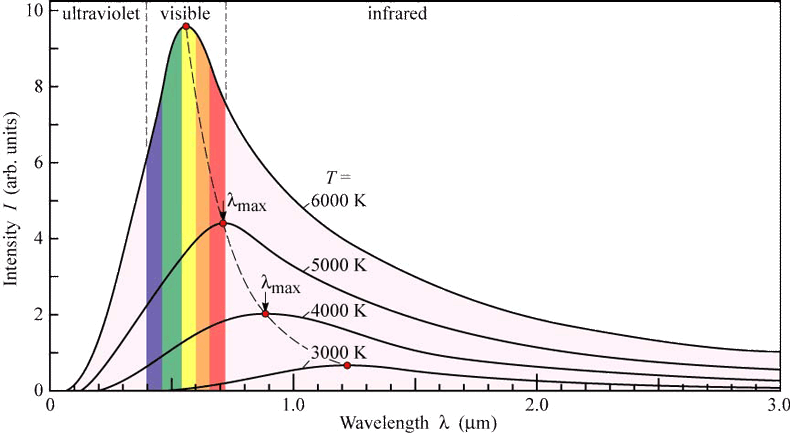
\includegraphics[width=\textwidth]{figures/exampleFigure.png}
% 	\caption{This is an example Figure.}
% 	\label{Figure in Chapter 1}
% \end{figure}

%% This is a table
% \begin{table}
% \caption{This is an example Table.}
% \begin{center}
% \begin{tabular}{ccc}
% x & f(x) & g(x) \\
% \hline
% 1 & 6 & 4  \\
% 2 & 6 & 3  \\
% 3 & 6 & 2  \\
% 4 & 6 & 2  \\
% \label{Table in Chapter 1}
% \end{tabular}
% \end{center}
% \end{table}


%%%%%%%%%%%%%%%%
% Chapter 2
%%%%%%%%%%%%%%%%

\chapter{Technical Approach}

\section{Background}
\subsection{Data-flow Analysis}
In compiler theory, data-flow analysis is a technique for gathering information about the possible set of values calculated at various points in a computer program. The basis for performing data-flow analysis is control flow graph (CFG), which is used to determine those parts of the program to which a particular value assigned to a variable might propagate. In our particular case, we used reaching-definition for each instruction to represent the data flow information. Two techniques applied for performing reaching-definition analysis are \textit{Liveness Analysis} and \textit{Reaching-Def Analysis}.

%CFG and ICFG
Control Flow Graph (CFG) is a graph representation of all the paths that a computer program might be traversed through during its execution. In a control flow graph, each node represents a basic block - a sequencial piece of a program that does not include jumps or jump targets, while the directed edges represent jumps in the program. Figure 2.1 is the complete control flow graph constructed for an example function t3f1. Each circle represents a basic block (first number in the circle denotes its line number), and the black edges represent the possible jumps that the program can take during execution. It is worth noting that the while loop in t3f1 includes a condition check at line 4, which can be reached from either line 4 (before loop starts) or from line 13 (after last instruction in the loop is finished). Therefore in the CFG there are two nodes representing line 5, with one coming from line 4 and another coming from line 13.

\begin{figure}
\begin{minipage}{\textwidth}
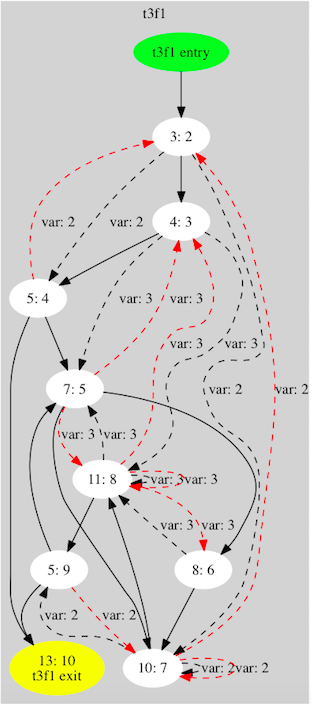
\includegraphics[width=0.6\textwidth]{figures/CFG.png}
\caption{Control Flow Graph for Function t3f1}
\label{CFG}
\end{minipage}
\end{figure}

\lstset{language=PHP}
\begin{minipage}{0.5\textwidth}
\begin{lstlisting}[frame=single]
<?php
function t3f1($c, $d) {
  $a = 0;
  $b = 0;
  while($a <= 5)
  {
    if ($b > 5) {
      $b = 5;
    }
    $a = $a + 1;
    $b = $b + 2;
  }
}
?>
\end{lstlisting}
\end{minipage}
\newline

%liveness analysis and reaching-def analysis
As one of the two techniques used for performing reaching-definition analysis, liveness analysis is to calculate, at instruction level, the variables that may be potentially read before their next write, that is, the variables that are live at the exit from each program point. In the given example, variable b is first defined at line 4; it is also defined at line 8 and 11 in the main loop. Therefore, var b is said to be "alive" from line 4 to line 8, and from line 11 back to line 8. Given liveness analysis output, def-use chains can be constructed for each variable. The DU chain represents the exact places where a variable definition is later used in other instructions. The DU chains in t3f1 are shown as black dotted edges in Figure 2.1.

To the contrary of liveness analysis, reaching-def analysis calculates the possible definition instructions for a given use variable. Reaching-def analysis helps generate use-def chains for each variable used in a program. The UD chains for variables in t3f1 are shown as red dotted edges in Figure 2.1.

\subsection{HipHop Bytecode}
\blindtext

\section{Inter-procedural CFG Construction}
Usually during static analysis, an intra-procedural CFG is constructed for each individual function before all intra-procedural CFGs are combined into one inter-procedural CFG (ICFG) that represents the control flow for the entire program. ICFG is a combination of all individual functions and a function call graph (CG), which is a graph representation of function dependencies in a program, in which functions are represented as nodes and function invokations are represented as directed edges. Since one variable defined/used in any function can be used/defined in other functions, extra work needs to be done in order to expand a variable's DU and UD chains in ICFG. Algorithm 1 shows the construction of DU and UD chains in ICFG given individual CFGs and CG.

\algdef{SE}[UNTIL]{Until}{EndUntil}[1]{\algorithmicuntil\ #1\ \algorithmicrepeat}{\algorithmicend\ \algorithmicuntil}%
\begin{algorithm}
\caption{Dataflow Expansion in ICFG}
\begin{algorithmic}[1]
\Require 
  \State $CG$: call graph of the application program; 
  \State $CFGS$: CFGs for all functions in the program

\Comment{main}
\Procedure{Dataflow Expansion}{}
\State{$visited$ $\gets$ $\emptyset$}
\For{Each $CFG$ in $CFGS$}
  \For{Each instruction $I$ in $CFG$}
    \If{$I$ has KILL variable $kv$}
      \State\Call{completeDefUse}{$CFG$, $I$, $kv$, $visited$}
    \EndIf
  \EndFor
\EndFor

\State{$visited$ $\gets$ $\emptyset$}

\For{Each $CFG$ in $CFGS$}
  \For{Each instruction $I$ in $CFG$}
    \If{$I$ has GEN variable $gv$}
      \State\Call{completeUseDef}{$CFG$, $I$, $gv$, $visited$}
    \EndIf
  \EndFor
\EndFor
\EndProcedure

\algstore{alg1}
\end{algorithmic}
\end{algorithm}

\begin{algorithm}
\begin{algorithmic}[1]
\algrestore{alg1}
\Function{completeDefUse}{$cfg$, $instr$, $var$, $visited$}
  \If{$instr$ in $visited$}
    \State\Return{$instr.duchain$}
  \EndIf
  \For{Each Use $use$ in $instr.duchain$}
    \If{$use$ is a function call site}
      \State Get the callee function $targetfunction$
      \State Get the function parameter $targetvar$ in $targetfunction$ that corresponds to $use.var$
      \State Get the instruction $targetInstr$ that initiates $targetvar$ in $targetfunction$
      \State $newuses$ $\gets$ \Call{completeDefUse}{$targetfunction.CFG$, $targetInstr$, $targetvar$, $visited$}
      \State $instr.duchain$ $\gets$ ($instr.duchain$ - $use$) $\cup$ $newuses$
    \EndIf
  \EndFor
  \State $visited$ $\gets$ $visited$ $\cup$ $instr$
  \State\Return{$instr.duchain$}
\EndFunction
\algstore{alg1}
\end{algorithmic}
\end{algorithm}

\begin{algorithm}
\begin{algorithmic}[1]
\algrestore{alg1}
\Function{completeUseDef}{cfg, instr, var, visited}
  \If{$instr$ in $visited$}
    \State\Return{$instr.udchain$}
  \EndIf
  \For{Each Def $def$ in $instr.udchain$}
    \If{$def$ is a function entry site}
      \State Get all the functions $callerfuncs$ that calls current function
      \For{Each function $callerfunc$ in $callerfuncs$}
        \State Get the function parameter $sourcevar$ in $callerfunc$ that corresponds to $def.var$
        \State Get the instruction $sourceInstr$ in $callerfunc$ that passes $sourcevar$ to callee stack
        \State $newdefs$ $\gets$ \Call{completeUseDef}{$callerfunc.CFG$, $sourceInstr$, $sourcevar$, $visited$}
        \State $instr.udchain$ $\gets$ ($instr.udchain$ - $def$) $\cup$ $newdefs$
      \EndFor
    \EndIf
  \EndFor
  \State $visited$ $\gets$ $visited$ $\cup$ $instr$
  \State\Return{$instr.duchain$}
\EndFunction
\end{algorithmic}
\end{algorithm}

\section{Testcase Generation Algorithm}

\subsection{Precise String Analysis for Input Generation}


\begin{table}
\begin{tabular}{c}
Supported PHP String Operations \\
\hline
Concat \\
StrComp \\
Substr \\
ToUpperCase \\
ToLowerCase \\
Reverse \\
Trim \\
Split \\
Replace \\
StrToTime \\
\label{Supported PHP string operations}
\end{tabular}
\end{table}

\subsection{Array Content Propagation}
\blindtext

\section{Interface Discovery Algorithm}
In this step, variables exposed by the application interface(input variables) are identified and grouped logically. This part of the program implements two interface discovery algorithms proposed by Halfond and Orso \cite{ref3}.



%%%%%%%%%%%%%%%%
% Chapter 3
%%%%%%%%%%%%%%%%

\chapter{Empirical Evaluation}

\section{Experiment Setup}
\subsection{Experimental Subjects}
The experimental subjects used in the study is consisted of three student-developed projects that use PHP as their backend language.

\subsection{Tools Used in Evaluation}
We evaluate the effectiveness of our interface discovery mechanism by comparing the number and quality of interfaces that it generates with the interfaces extracted by web crawlers. The web crawler tool that we used is OpenWebSpider, an open-sourced framework for crawling/spidering websites. For each interface output, we check if any of the HTTP requests in this output is processed in the backend program.

We evaluate the effectiveness of our test request generation mechanism by comparing it against another PHP test case generation tool, PHPUnit. For each HTTP request, a set of possible values is generated for all of the fields in this request, creating a set of test HTTP requests, which are then sent to the server. Then the final code coverage in the backend is recorded.

\section{Results}

%example%
\subsection{Email Sender}
A simple PHP program that processes a form which contains 4 input fields and sends an email according to the information supplied in the form. 

Form Inputs
\begin{itemize}
\item first\_name (required)
\item last\_name (required)
\item email (required)
\item telephone (optional)
\end{itemize}
All required fields are checked against a regular expression. The only optional field (telephone) is not checked against any regex or string variables.

Our penetration testing tool successfully identified all the fields (required and optional). It generated test cases for all the required variables from the given regex expression. For the "telephone" field, which is optional, our testing tool did not infer any information from static analysis, therefore would be producing random strings for this field during testing.

%example%
\subsection{Fancy Hotel (CS4400 Class Project)}
A web application powered by PHP and MySQL that serves as an online room reservation system for a non-existing hotel.

\subsubsection{User Login}
Form Inputs
\begin{itemize}
\item username (string)
\item password (string)
\end{itemize}

Our penetration testing tool successfully identified both username and password fields in the interface. Since the application does not compare username and password to specific patterns or values, our static analysis did not infer possible value information for these fields. 

However, the analyzer identified session information created during login, which could potentially make subsequent penetration testing more thorough by exploiting user sessions.

In addition, the user login program can be redirected to three different URLs once login information is validated. Since these URLs are not exposed to the front-end HTML, they were not identified by webcrawler. However, by performing static analysis on the source code, our penetration testing tool was able to discover all three of them.

\subsubsection{User Registration}
Form Inputs
\begin{itemize}
\item username (string)
\item password (string)
\item confirmed\_password (string)
\item email (string)
\end{itemize}

Our penetration tool successfully identified all request (or interface) parameters and their names (usn, psw, con\_pwd, email). It identified the regular expression that was used to check valid email and username in the program and used this information to construct test cases for the email and username fields.

\subsubsection{Room Search}
Form Inputs
\begin{itemize}
  \item start\_date (string)
  \item end\_date (string)
  \item location (string)
\end{itemize}

Note
\begin{itemize}
\item start\_date must be greater than 2015-08-01;
\item start\_date cannot be greater than end\_date;
\item start\_date cannot be smaller than today’s date (2015-08-31);
\item end\_date must be smaller than 2016-01-31;
\end{itemize}

Our penetration tester successfully identified all the required fields as well as the session information not exposed by the interface itself. Furthermore, static analysis has inferred key information about both start\_date and end\_date. For start\_date, output test cases include "2015\-08\-31" and "2015\-08\-01"; for end\_date, output test cases include "2016\-01\-31". 

%example%
\subsection{Paycheck Calculator}
A basic PHP web application that takes in one input (salary) and shows how much tax should be deduced.

Form Inputs
\begin{itemize}
  \item salary (float)
\end{itemize}

Our penetration tool successfully identified the interface. Static analysis generated all possible levels of salary which covered 100\% of application code.






%%%%%%%%%%%%%%%%
% Chapter 4
%%%%%%%%%%%%%%%%

\chapter{Discussion}
Lorem ipsum dolor sit amet, consectetur adipiscing elit, sed do eiusmod tempor incididunt ut labore et dolore magna aliqua. Ut enim ad minim veniam, quis nostrud exercitation ullamco laboris nisi ut aliquip ex ea commodo consequat. Duis aute irure dolor in reprehenderit in voluptate velit esse cillum dolore eu fugiat nulla pariatur. Excepteur sint occaecat cupidatat non proident, sunt in culpa qui officia deserunt mollit anim id est laborum..


%%%%%%%%%%%%%%%%
% Chapter 5
%%%%%%%%%%%%%%%%

\chapter{Conclusion}
In this paper we presented a novel approach for performing automated penetration testing for PHP web applications. It uses static analysis to identify the application program's behavior on each variable and function, and then construct the possible interfaces exposed by the application as well as the possible values that each request field can take. We compared the effectiveness of this new test system with traditional penetration testing tools, in terms of interface discovery and test case generation. The result shows our proposed testing tool can not only identify more interfaces for dynamic web applications, but also generate fewer test cases in order to cover 100\% of the backend code.

%%%%%%%%%%%%%%%%
% Appendices
%%%%%%%%%%%%%%%%

\begin{appendices}

%Some Table of Contents entry formatting
\addtocontents{toc}{\protect\renewcommand{\protect\cftchappresnum}{\appendixname\space}}
\addtocontents{toc}{\protect\renewcommand{\protect\cftchapnumwidth}{6em}}

%Begin individual appendices, separated as chapters

\chapter{Experiment Equipment}
\begin{enumerate}
\item Ubuntu 14.04
\item Java Runtime Environment 1.7
\item PHP 5.5
\item HHVM 3.10.0
\item OpenWebSpider
\end{enumerate}

\chapter{Algorithm}
\label{appendix:algorithm}



\end{appendices}

%%%%%%%%%%%%%%%%
% References
%%%%%%%%%%%%%%%%

\begin{singlespace}  % use single-line spacing for multi-line text within a single reference
	\setlength\bibitemsep{\baselineskip}  %manually set separataion betwen items in bibliography to double space
	\appto{\bibsetup}{\raggedright}
  \printbibliography[title={References}]
\end{singlespace}

\addcontentsline{toc}{chapter}{References}  %add References section to Table of Contents


\end{document}
